\documentclass[10pt,t,aspectratio=169]{beamer}

\usetheme[progressbar=frametitle]{moloch}

%\usepackage{helvet}
%\usepackage[sfdefault,light]{FiraSans}
\usepackage[sfdefault]{inter}

\usepackage[T1]{fontenc}
\usepackage[latin9]{inputenc}
\usepackage{amssymb}
\PassOptionsToPackage{no-math}{fontspec}
\usepackage{graphicx} 
\usepackage{hyperref} 
\usepackage{multirow} 
\usepackage{xspace}
\usepackage{booktabs}

\usepackage{environ,adjustbox}
% 1) Gather the body of every table environment in \BODY
% 2) Replace it by an adjustbox of at most \textwidth
\RenewEnviron{table}{%
  \begin{adjustbox}{max width=\textwidth,center}%
    \BODY
  \end{adjustbox}%
}


\usepackage{siunitx}
\usepackage{tabularray}
\UseTblrLibrary{booktabs,siunitx,longtable}

\setbeamercolor{normal text}{fg=mDarkTeal,bg=white}
\definecolor{cardinalred}{rgb}{0.549, 0.082, 0.082}
\setbeamercolor{progress bar}{ fg = white }
\setbeamercolor{title separator}{ fg = cardinalred}
\setbeamercolor{progress bar in section page}{ fg = cardinalred }

\newtheorem{proposition}{Proposition} 

\title{O Praeclarum Titulum}
\subtitle{Lorem ipsum dolor}
% \date{\today}
\date{}
\author{Author 1 (Affiliation) \\
        Author 2 (Affiliation)}

\begin{document}

\maketitle

\begin{frame}{Motivation}

    motivation

\end{frame}

\begin{frame}{This paper}

    this paper
  
\end{frame}

\section{Background}

\begin{frame}{xxx}

    xxx
  
\end{frame}

\section{Data}

\begin{frame}{xxx}

    xxx
  
\end{frame}

\section{Results}

\begin{frame}{xxx}

    \begin{table}
\centering
\begin{talltblr}[         %% tabularray outer open
caption={Results},
]                     %% tabularray outer close
{                     %% tabularray inner open
colspec={Q[]Q[]Q[]Q[]},
column{2,3,4}={}{halign=c,},
column{1}={}{halign=l,},
hline{8}={1,2,3,4}{solid, black, 0.05em},
}                     %% tabularray inner close
\toprule
& City FE & Highway FE & Both \\ \midrule %% TinyTableHeader
(Intercept) & \num{7.558} & \num{7.368} & \num{7.565} \\
& (\num{0.521}) & (\num{0.306}) & (\num{0.453}) \\
cty & \num{-0.242} &  & \num{-0.233} \\
& (\num{0.022}) &  & (\num{0.127}) \\
hwy &  & \num{-0.166} & \num{-0.007} \\
&  & (\num{0.005}) & (\num{0.079}) \\
Num.Obs. & \num{234} & \num{234} & \num{234} \\
R2 & \num{0.638} & \num{0.587} & \num{0.638} \\
R2 Adj. & \num{0.636} & \num{0.585} & \num{0.635} \\
Std.Errors & by: year & by: year & by: year \\
\bottomrule
\end{talltblr}
\end{table}


\end{frame}

\begin{frame}{xxx}
    \centering
    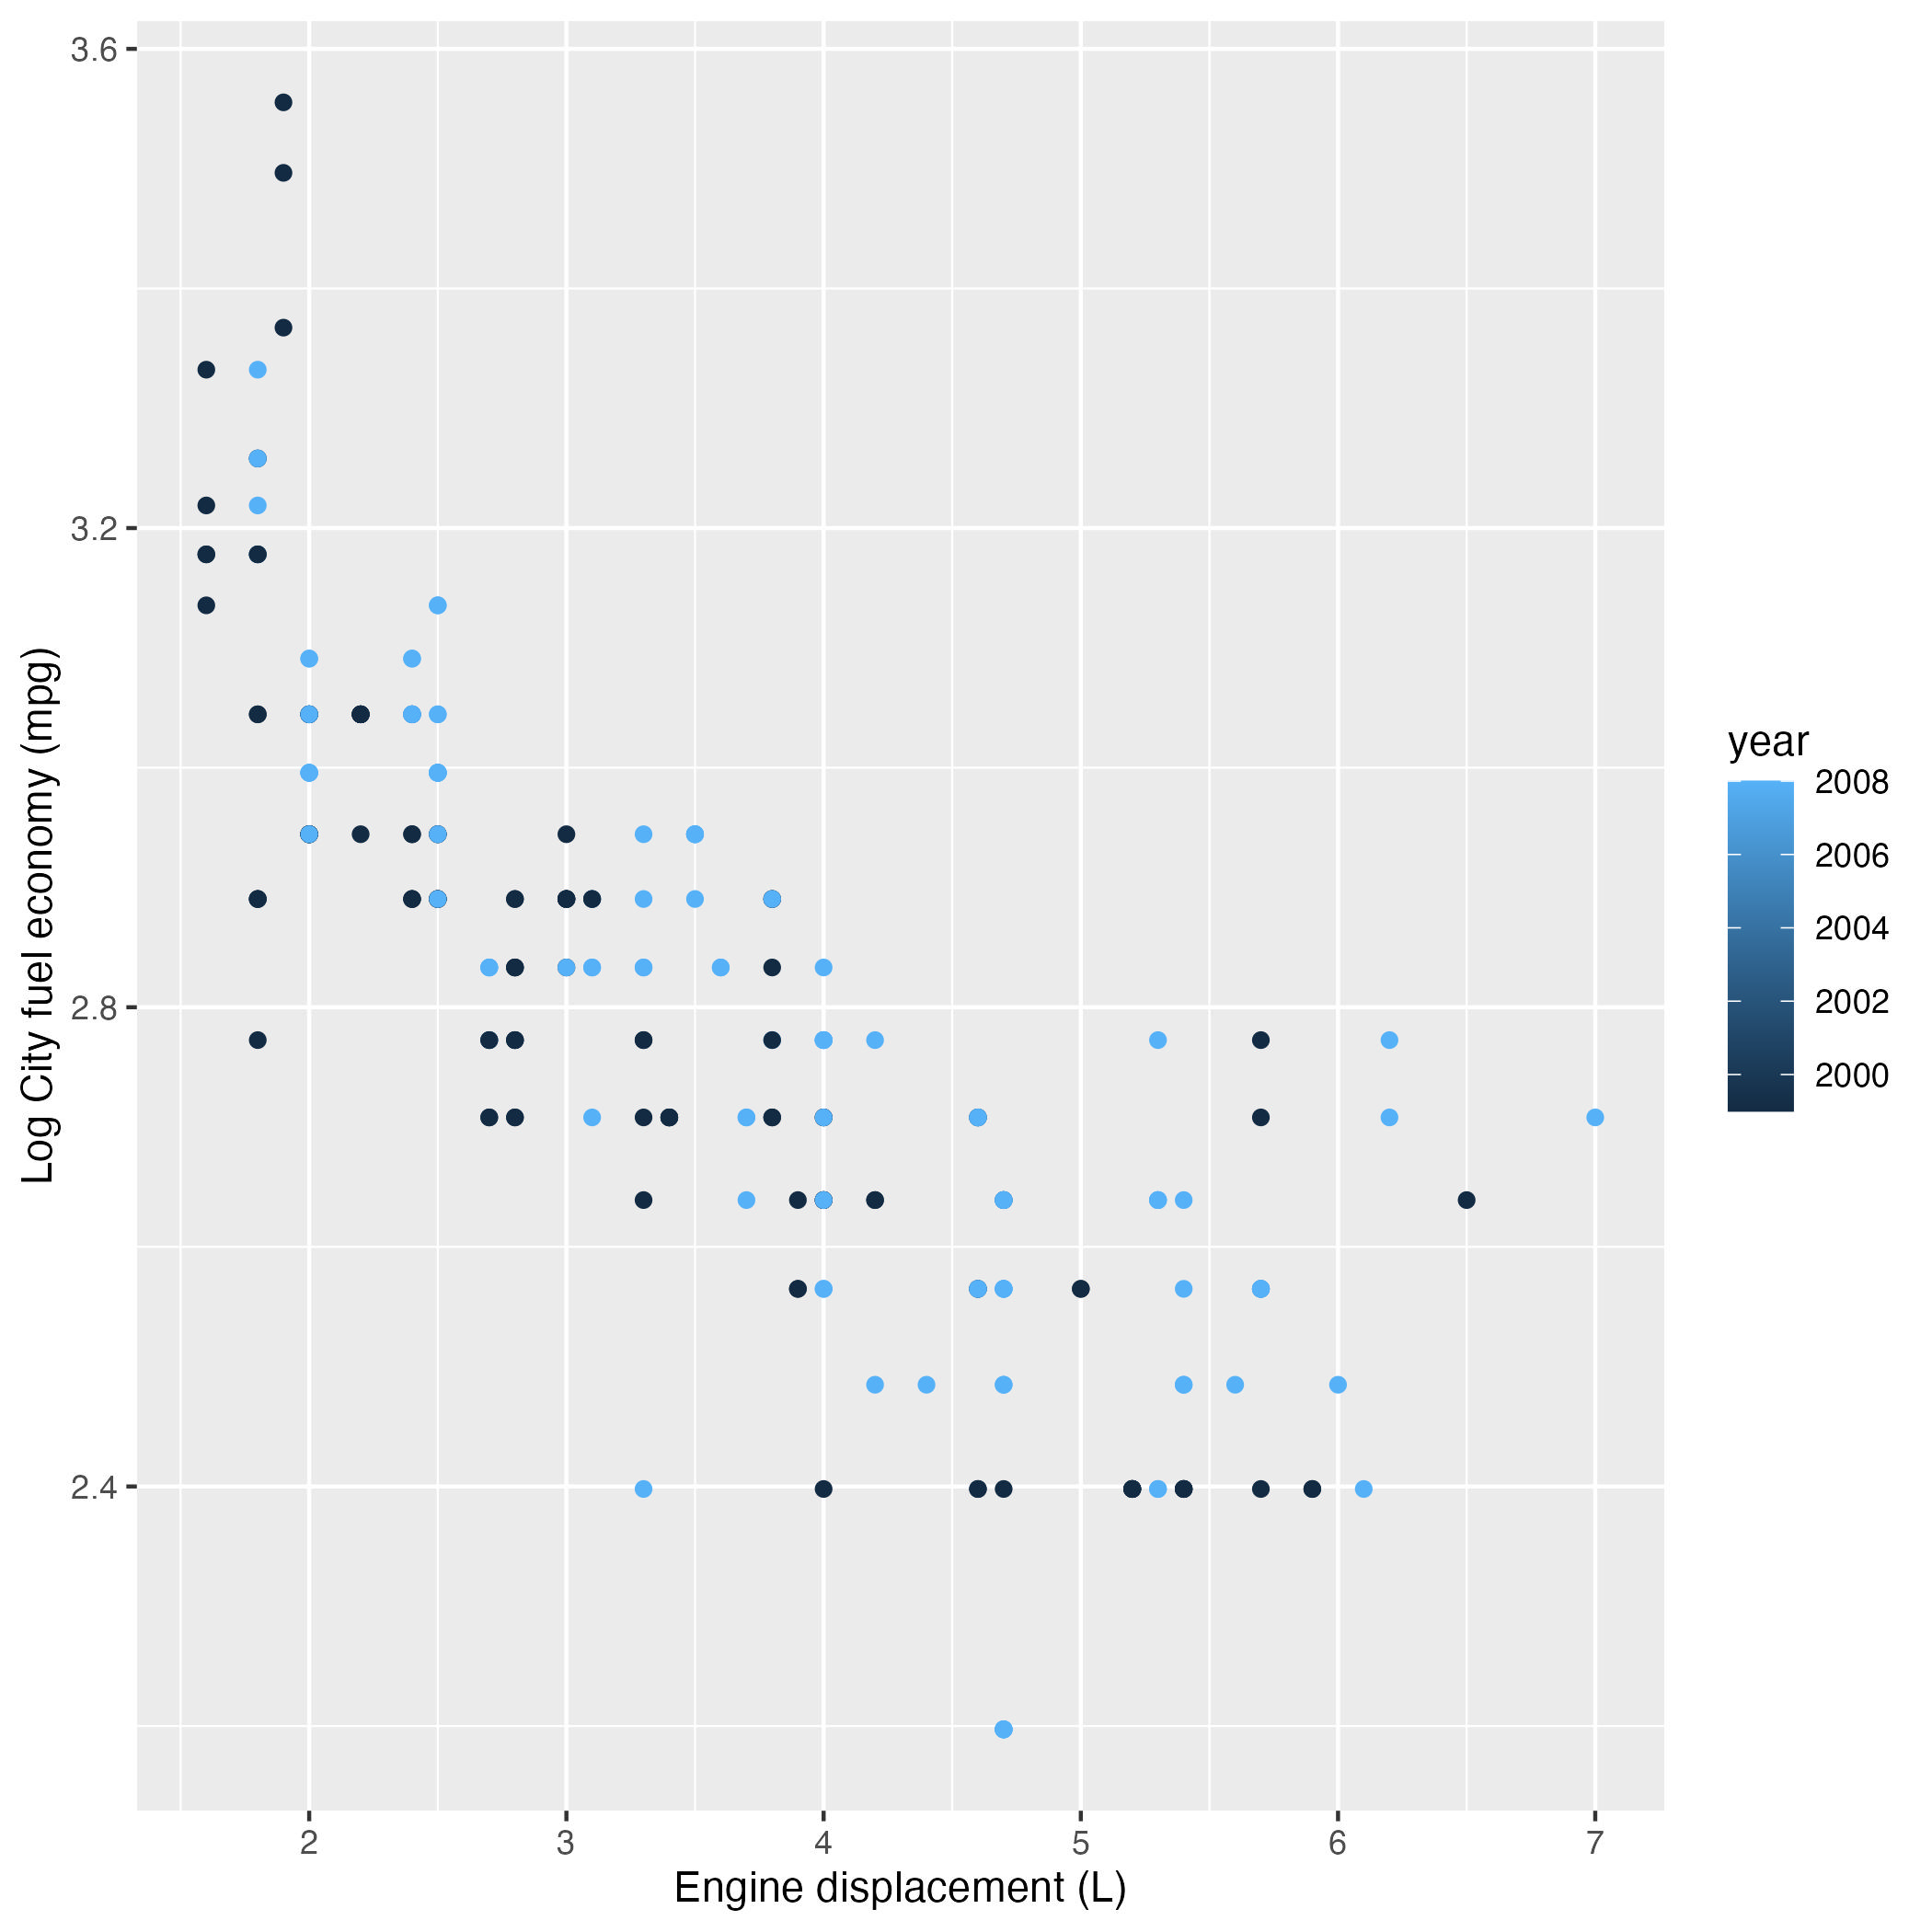
\includegraphics[width=0.5\linewidth]{../input/figure_city.jpg}
  
\end{frame}

\section{Conclusion}

\begin{frame}{xxx}

    xxx
  
\end{frame}

\end{document}
